\documentclass[../../../interview-questions.tex]{subfiles}

\begin{document}

\subsection{MySQL之InnoDB内存结构}

Innodb的内存结构主要分为 3 个部分: Buffer Pool、Change Buffer、Adaptive Hash Index,另外还有一个(redo)log buffer。MySQL 8.0内存结构如图\ref{fig:innodbmemory}所示,官方地址\footnote{\url{https://dev.mysql.com/doc/refman/8.0/en/innodb-architecture.html}}。

\begin{figure}[htbp]
    \centering
    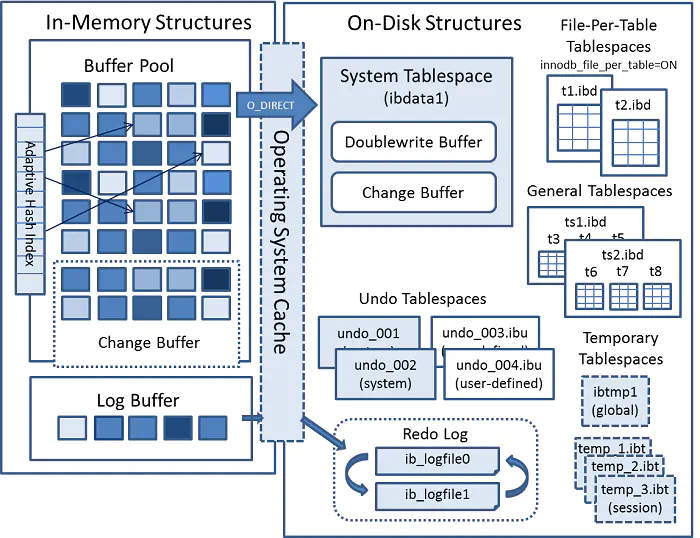
\includegraphics[scale=0.35]{innodbpng.png}
    \caption{InnoDB 8.0内存磁盘结构}
    \label{fig:innodbmemory}
\end{figure}

\paragraph{缓冲池 Buffer Pool}

首先,InnnoDB的数据都是放在磁盘上的,InnoDB操作数据有一个最小的逻辑单位,叫做页(索引页和数据页)。我们对于数据的操作,不是每次都直接操作磁盘,因为磁盘的速度太慢了。 InnoDB使用了一种缓冲池的技术,也就是把磁盘读到的页放到一块内存区域里面。这个内存区域就叫Buffer Pool。下一次读取相同的页,先判断是不是在缓冲池里面,如果是,就直接读取,不用再次访问磁盘。修改数据的时候,先修改缓冲池里面的页。内存的数据页和磁盘数据不一致的时候,我们把它叫做脏页。InnoDB里面有专门的后台线程把Buffer Pool的数据写入到磁盘,每隔一段时间就一次性地把多个修改写入磁盘,这个动作就叫做刷脏。Buffer Pool缓存的是页面信息,包括数据页、索引页。Buffer Pool默认大小是128M(134217728字节),可以调整。

\paragraph{Change Buffer(写缓冲)}

如果这个数据页不是唯一索引(注:唯一索引就是在同一字段下不能有相同值),也就不需要从磁盘加载索引页判断数据是不是重复(唯一性检查)。这种情况下可以先把修改记录在内存的缓冲池中,从而提升更新语句(Insert、Delete、Update)的执行速度。这一块区域就是 Change Buffer。5.5 之前叫Insert Buffer 插入缓冲,现在也能支持delete和update。最后把 Change Buffer 记录到数据页的操作叫做 merge。

什么时候发生 merge?有几种情况:在访问这个数据页的时候,或者通过后台线程、或者数据库shut down、redo log写满时触发。

\paragraph{(redo) Log Buffer}

思考一个问题:如果BufferPool里面的脏页还没有刷入磁盘时,数据库宕机或者重启,这些数据丢失。如果写操作写到一半,甚至可能会破坏数据文件导致数据库不可用。为了避免这个问题, InnoDB把所有对页面的修改操作专门写入一个日志文件,并且在数据库启动时从这个文件进行恢复操作(实现crash-safe)——用它来实现事务的持久性。这个文件就是磁盘的redo log(叫做重做日志),对应于/var/lib/mysql/目录下的ib\_logfile0和ib\_logfile1,每个48M。 这种日志和磁盘配合的整个过程,其实就是 MySQL 里的 WAL 技术(Write-Ahead Logging),它的关键点就是先写日志,再写磁盘。

https://www.cnblogs.com/tracydzf/p/15788762.html



\end{document}